\documentclass[10pt,a4paper,oneside]{memoir}

\usepackage{a4wide}
\usepackage[utf8]{inputenc}
\usepackage[T1]{fontenc}
\usepackage{a4}
\usepackage{color}
%\usepackage{geometry}
\usepackage[francais]{babel}
\usepackage{hyperref}
\usepackage{listings}
%\usepackage{latexsym}
%\usepackage{graphicx}
%\usepackage{appendix}
\usepackage{fancybox}
\usepackage{url}
\usepackage{graphics}
\usepackage{graphicx}
%\usepackage{harvard}
\urlstyle{sf}
\makeatletter\def\input@path{{contenu/}{src/}{eps/}}\makeatother


\newcommand{\crypt}[2]{\begin{center}\texttt{#1}\ \ $\Longrightarrow$\ \ \texttt{#2}\end{center}}
\newenvironment{fminipage}%
  {\begin{center}\begin{Sbox}\begin{minipage}{1\textwidth}}%
  {\end{minipage}\end{Sbox}\fbox{\TheSbox}\end{center}}
\newcommand{\definition}[1]{\begin{center}#1\end{center}}
\renewcommand{\footref}[1]{\footnote{voir chapitre \ref{#1}, page
    \pageref{#1}}}
\newcommand{\note}[1]{\begin{center}\begin{minipage}{0.7\textwidth}\textsc{Note
          : }#1\end{minipage}\end{center}}
\newcommand{\bc}[1]{#1\ieme~ siècle avant J.-C.}


%\setlength{\voffset}{-0.9in}
%\setlength{\hoffset}{-0.5in}
%\setlength{\textwidth}{6.5in}
%\setlength{\textheight}{10.5in}

\title{Travail de fin d'études \\
  \textbf{La cryptographie} \\ 
  Peut on réellement cacher des informations ?}
\author{Quentin Stiévenart\\
Athéné Royal de Waterloo}
\date{Année scolaire 2008 - 2009}


\pagestyle{headings}
\begin{document}
% Titre, table des matières
\frontmatter
\maketitle \clearpage
\tableofcontents \clearpage

% Introduction
\chapter{Introduction}
\thispagestyle{empty}

\section{Présentation du travail}
La cryptographie fait aujourd'hui partie de la vie de tous les jours,
on l'utilise sans le savoir, principalement en naviguant sur internet
(via les connexions sécurisées, les envois de mails chiffrés\dots).

Mais qu'est-ce que la cryptographie ? Comment cela
fonctionne-t-il ? Son utilisation se limite-t-elle à l'informatique ?
Depuis quand existe la cryptographie ?

C'est à ces questions que nous allons essayer de répondre durant ce
travail, et plus principalement à celle-ci :

\begin{quote}
\emph{«~Peut-on réellement cacher des informations ?~»}
\end{quote}

Nous essayerons donc de savoir si l'on peut, et comment on peut 
envoyer sans risque une information, un message, des données\dots à
quelqu'un, sans qu'une personne extérieure puisse le lire.

Pour répondre à ces questions, nous allons tout d'abord parler de
l'utilisation  de la cryptographie
à travers l'histoire, pour présenter ensuite les
différentes techniques existantes. Nous parlerons
aussi du moyen de « contrer » la cryptographie, avec la
cryptanalyse. Nous verrons enfin ce qu'il en est de la
cryptographie de nos jours. 

% La cryptographie est, comme le dit si bien Lacroix dans le titre de
% son livre ``La cryptographie, ou l'art d'écrire en chiffres''
% \cite{ArtDecrireEnChiffres},
% un ensemble de méthodes mathématiques ou autres, par lesquelles on va ``crypter'' un message, de façon à le rendre illisible si on n'a pas connaissance de la méthode utilisée, ou de l'éventuelle clée utilisée. \\
% Ce travail aura pour but de savoir si la cryptographie est un moyen fiable pour cacher des données, via l'analyse de certains algorithmes utilisés de nos jours ou dans le passé, et plus précisément leur cryptanalyse (ce terme sera définit à la prochaine section du document) \\
% Nous analyserons donc, d'abord les méthodes de cryptographie utilisée dans l'histoire, suivant un ordre chronologique, ensuite nous passerons aux méthodes actuelles, où nous expliquerons entre autres l'utilité de la cryptographie de nos jours. \\

%En annexe, on pourra voir quelques implémentations d'algorithmes de chiffrement dans certains langages de programmation (Haskell, C, Common Lisp, Python)\footnote{Pour plus d'infos sur ces langages, visitez respectivement \url{http://www.haskell.org}, \url{http://fr.wikipedia.org/wiki/Langage_C}, \url{http://cliki.net} et \url{http://www.python.org}.} \\

\section{Mes motivations pour ce travail}
J'ai choisi de faire un travail de fin d'études sur la cryptographie
car j'ai toujours été intéressé par les mathématiques et surtout par
l'informatique (plus le fonctionnement de l'ordinateur et sa
programmation, que l'aspect « jeux et divertissements » de
l'informatique, ainsi que la sécurité informatique)~;
la cryptographie fait partie intégrante des
systèmes informatiques d'aujourd'hui et est basée sur des principes
mathématiques. Je compte d'ailleurs faire des études polytechniques
l'année prochaine. \\ L'idée de ce travail m'est venue petit à
petit. Après la lecture d'un article sur la cryptographie sur
internet, j'ai commencé à m'y intéresser un peu, mais sans plus.
 Ce travail me permet donc d'approfondir le sujet.

\section{À propos de ce document}
Pour des raisons personnelles et dans un esprit de liberté de
l'information, ce document est placé sous licence Creative Commons
BY-SA\footnote{\url{http://creativecommons.org/licenses/by-sa/2.0/fr/}}, ce qui
signifie que vous pouvez le modifier et le redistribuer librement à
condition de préciser le nom de l'auteur, et de garder cette même
licence. Toujours pour les mêmes raisons, ce document a été préparé à
l'aide d'outils entièrement libres.
%de l'éditeur de texte \texttt{GNU
%  Emacs} et du logiciel de composition typographique \LaTeX, et des
%logiciels \texttt{xfig}, \texttt{dia} et \texttt{inkscape} pour les
%dessins, sur un système d'exploitation basé sur \texttt{Linux}. Tous
%ces logiciels sont entièrement libres. De plus, les langages utilisés
%en annexe possèdent aussi chacun au moins une implémentation
%libre.
Pour plus d'informations sur les logiciels libres et la culture
libre, référez-vous à \url{http://www.gnu.org/philosophy/philosophy.fr.html}. \\
Ce document, ses sources (les fichiers \TeX, les graphiques, et les
codes sources des annexes), ainsi que des informations supplémentaires
sont disponibles sur internet via l'adresse
\url{http://acieroid.tuxfamily.org/crypto}. \\


\section{Présentation de la cryptologie}
Étymologiquement, la cryptologie signifie la «~science du secret~»~;
elle consiste à cacher une
information, un message ou de quelconques données via la
\emph{cryptographie}. Nous étudierons son histoire
dans le chapitre \ref{chap:Histoire}.

La cryptographie comprend des méthodes très variées (des
\emph{systèmes de chiffrement} pour rendre les messages chiffrés),
certaines méthodes étant plus efficaces que les autres.
Nous examinerons ces méthodes dans le chapitre
\ref{chap:Techniques}.

La cryptologie comprend aussi la \emph{cryptanalyse}, qui consiste à
retrouver le message d'origine à partir d'un message chiffré sans en
connaître la clé ou le secret utilisé pour chiffrer le message.
Nous verrons cet aspect dans le chapitre \ref{chap:Cryptanalyse}.

Au cours de ce travail, nous utiliserons de nombreux termes se référant à
la cryptologie. \\
Définissons-en quelques uns : 

%\newcommand{\glossaire}[2]{\nomenclature{\textbf{#1}}{#2}}
\begin{itemize}

\item \sffamily{\textbf{le chiffrement}} est la démarche effectuée afin de rendre
  le message clair illisible, chiffré. On utilise parfois le terme
  «~cryptage~», qui est un anglicisme, nous éviterons donc de
  l'utiliser~;

\item \sffamily{\textbf{le déchiffrement}} est la démarche inverse du chiffrement, qui retrouve
  le message clair à partir du message chiffré en ayant connaissance
  de la clé, du secret ou de l'algorithme utilisé (contrairement à la
  cryptanalyse). Le mot \sffamily{\textbf{décryptage}} peut aussi
être utilisé~;
\item \sffamily{\textbf{la cryptanalyse}} vise à retrouver le
message clair à partir du message chiffré sans avoir connaissance
de la clé ou du secret~;

\item \sffamily\textbf{{la stéganographie}} est une discipline semblable à la
  cryptographie mais qui consiste à cacher un message (dans une
  image, \dots) et non pas à la rendre initelligible. Nous ne
développerons donc pas ce sujet ici~;

\item \sffamily\textbf{{la clé de chiffrement}} est une donnée (mot, suite d'opération,
  nombre, \dots) utilisée pendant le chiffrement afin de rendre le
  déchiffrement plus difficile sans la connaissance de celle-ci. Il
  existe plusieurs types de clés : certaines qui doivent être gardées
  secrètes (clés privées) et d'autres qui peuvent être diffusées
  (clés publiques)~;

\item \sffamily\textbf{{les données claires}} sont les données dans leur forme initiale, non
  chiffrées. Ces données peuvent être du texte (un message) ou d'autres
  données informatiques (un fichier, \dots)~;

\item \sffamily\textbf{{les données chiffrées}} sont données qui
sont chiffrées via un certain
  algorithme de chiffrement~;

\item \sffamily\textbf{{un cryptogramme}} est un message chiffré
dans le but d'être déchiffré par des amateurs de cryptographie (on
en retrouve par exemple dans les journaux. Ils sont la plupart du
temps assez simples.

\end{itemize}



% Partie principale
\mainmatter

\chapter{Présentation de la cryptologie}
\section{Qu'est ce que la cryptologie}
La cryptologie est la « science du secret », et consiste a cacher une
information, un message, ou de quelconques données via la
\emph{cryptographie}. 

Elle comprends aussi la \emph{cryptanalyse}, qui consiste à retrouver
le message d'origine à partir d'un message chiffré, sans en connaître
la clé ou le secret utilisé pour chiffrer le message.
\section{Vocabulaire\label{s:Definitions}}
Avant toute chose, il est nécéssaire de définir quelques termes pour
les clarifier dans l'esprit de chacun, et pour éviter de les confondre
:
\begin{itemize}
\renewcommand{\makelabel}[1]{\sffamily\textbf{#1}}
\item[Le chiffrement] se réfère à la démarche effectuée afin de rendre
  le message clair illisible, chiffré. On utilise parfois le terme
  « cryptage », qui est un anglicisme, nous éviterons donc de
  l'utiliser ;

\item[Le déchiffrement, ou décryptage] est le sens inverse du
  chiffrement, qui retrouve le message clair à partir du message
  chiffré, en ayant connaissance de la clé, du secret ou de
  l'algorithme utilisé (contrairement à la cryptanalyse). Le terme
  « décryptage » est un terme français correct, contrairement au
  « cryptage » ;

\item[La stéganographie] est une discipline semblable à la
  cryptographie, mais qui consiste à « cacher » un message (dans une
  image, ...) et non pas à le rendre inintelligible. Ce sujet étant
  tout aussi vaste que la cryptographie, nous ne l'étudierons pas dans
  ce travail ;

\item[La clé de chiffrement] est une donnée (mot, suite d'opération,
  nombre, ...) utilisée pendant le chiffrement afin de rendre le
  déchiffrement plus difficile sans la connaissance de celle ci.
  Nous verrons qu'il existe deux types de clés : \emph{symétrique}
  (\emph{privées}) et \emph{asymétrique} (\emph{publiques}), et que
  l'utilisation de clé est crucial dans la cryptographie actuelle.
\end{itemize}

\section{Règles typographiques}
Tout au long de ce travail, nous allons utiliser certaines notations : 
\begin{itemize}
\item Une \textbf{clé de chiffrement} sera notée $k$ (pour «  Key  »,
  «  Clé  » en anglais), indicé si nous utilisons plusieurs clés ;
  \item Un \textbf{message en clair} sera noté $M$ (pour «  Message  ») ;
  \item Un \textbf{message chiffré} sera noté $C$ (pour «  Chiffré  ») ;
  \item Une \textbf{fonction de chiffrement} $e$ (pour « Encryption
    », «  Chiffrage  » en anglais) ou $e_k$, selon qu'elle utilise
    une clé pour le chiffrement ;
  \item Une \textbf{fonction de déchiffrement} $d$ (pour
    « Decryption », « Déchiffrement  » en anglais) ou $d_k$,
    similairement à la fonction de chiffrement.
\end{itemize}
L'opération de chiffrement se notera alors comme suit pour un
algorithme de chiffrement avec une clé.
\begin{center}
  \begin{math}
    e_k(M) = C
  \end{math}
\end{center}
Et l'opération de déchiffrement se notera ainsi :
\begin{center}
  \begin{math}
    d_k(C) = M
  \end{math}
\end{center}
Nous utiliserons aussi la notation : 
\crypt{Cryptographie}{Pelcgbtencuvr}
pour indiquer que le mot « Cryptographie » sera chiffré en
 « Pelcgbtencuvr ». 
  

\chapter{La cryptographie à travers l'histoire}
Avant de commencer à décrire la cryptographie en soit, voyons un peu
son histoire, son apparition, et son évolution au fil du temps.

\section{L'apparition de la cryptographie}
La cryptographie serait apparue pour la première fois il y a 4000 ans,
au bord du Nil, où un scribe aurait tracé d'une façon spéciale des
hiérogliphes sur la tombe de son maître, bien que ce n'était pas
vraiment dans le but de rendre le texte illisible, mais de le rendre
plus solennel. \\

La seconde trace de cryptographie date du \bc{XVI}, c'est une tablette
d'argile sur laquelle un potier aurait écrit sa recette en enlevant
les consonnes et en changeant l'orthographe de certains mots. \\

À cette époque là, les seuls moyens utilisés pour cacher les messages
ressemblaient plus à de la stéganographie qu'à de la cryptographie,
les messages ne sont pas rendus illisibles, mais sont cachés. Par
exemple, aux de -600, Nabuchodonosor rasait le crâne d'un esclave,
écrivait un message dessus, et une fois que les cheveux avaient
repoussés, l'esclave allait chez le destinataire du message, qui lui
rasait les cheveux pour le lire. Un autre exemple est celui d'Harpage,
qui était chargé de tuer Cyrus, le petit fils du roi de Mèdes, mais
qui ne le fait pas. Par la suite, quand Cyrus aura grandit, pour
communiquer avec lui, Harpage cache les lettres dans le ventre de
lièvres, qu'il recouds par la suite. De cette façon, le message passe
inaperçu. \\

Les premières « vraies » techniques de cryptographie apparaissent
quant à elles à partir du \bc{VI}, avec une méthode de substitution,
nommée \emph{atbash}, qui consiste à remplacer les lettres par la
lettre « opposée », c'est-à-dire que A sera remplacé par Z, B par Y,
et ainsi de suite. \\

\begin{figure}[h]
  \begin{center}
    \includegraphics[scale=0.15]{eps/scytale}
  \end{center}
  \caption{La scytale des spartiates (\bc{V})}
  \label{fig:scytale}
\end{figure}
  
Ensuite, au \bc{V}, les spartiates utilisaient pour communiquer le
bâton de Plutarque, plus connu sous le nom de \emph{scytale}. Cette
technique consistait à enrouler un long et étroit morceau de parchemin
autour d'un bâton, on écrivait ensuite le message sur le parchemin, et
on envoyait ce parchemin déroulé au destinataire, qui possédait un
bâton
de même diamètre pour déchiffrer le message. \\

Le premier réel système cryptographique par substitution est inventé
par un historien grec, Polybe aux alentours de 150 avant J.-C. (nous
verrons ce système en détail dans le chapitre \ref{syst:carrepolybe} (page
\pageref{syst:carrepolybe}). \\

\label{syst:chiffrecesar}
Pendant le \bc{I}, les armées de César utilisaient une méthode de
chiffrement par substitution simple, qui consistait à décaler les
lettres de l'alphabet d'un certain rang dans l'alphabet (de 3 rangs la
plupart du temps, ainsi A devient D, B devient E, \dots). Cette simple
méthode est une des méthodes de chiffrement les plus connues et à été
utilisées de nombreuses fois par la suite dans des formes dérivées (chiffre de
Vigenère\footref{syst:chiffrevigenere}, rot13\footref{syst:rot13}), ou même
de la même façon (pendant la guerre de sécession par exemple)

\begin{figure}[h]
  \begin{center}
    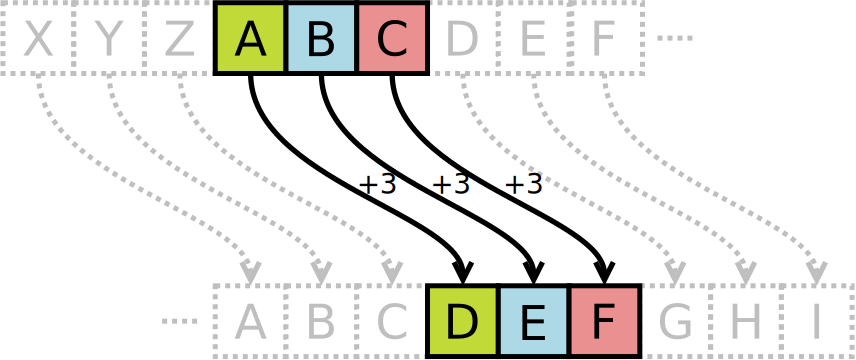
\includegraphics[scale=0.4]{eps/chiffrecesar}
  \end{center}
  \caption{Le chiffre de César}
  \label{fig:chiffrecesar}
\end{figure}

Au Moyen-âge, comme la plupart des sciences, la cryptologie n'évolue
presque pas (une personne pratiquant la cryptologie peut être
considéré comme faisant de la magie noire), à part quelques exceptions
au Moyen-Orient et en Asie (dans le Kama-sutra, il est dit que les
femmes doivent apprendre le \emph{mlecchita-vikalpa} (l'art de
l'écriture secrète) pour cacher leurs liaisons.). Il faut donc
attendre le XV\ieme~ siècle pour que la cryptographie commence
réellement à évoluer. \\

\section{L'évolution de la cryptographie}
Au début du XV\ieme~ siècle donc, un égyptien écrit une encyclopédie en
24 volumes comprenant une partie sur la cryptologie qui décrit des
chiffres de substitution et de transposition. Le premier chiffre de
substitution polyalphabétique\footref{substitutionpolyalphabetique}
est inventé par Leone Battista Alberti en 1467, un humaniste italien
de la reinaissance, aussi connu pour ses travaux en architecture,
surnommé \emph{Le père de la cryptographie occidentale} par
l'historien David Kahn\cite{Codebreakers}. Cette technique est appelée
le \emph{cadran chiffran}\label{syst:cadranchiffran}, ce sont deux
disques de 24 cases attachés, contenant les lettres de l'alphabet (le
premier en contient 20, H, K et Y n'étant pas « indispensables », J, U
et W n'étant pas dans l'alphabet latin, les 4 autres cases sont
occupées par des chiffres. L'autre disque contient les 23 lettres
latines dans un ordre aléatoire et le signe \&). Le plus petit disque
peut tourner, les lettres claires et chiffrées se trouvent alors face
à face, et il suffit de recopier la lettre du petit disque pour
chiffrer la lettre du grand disque. Après avoir chiffré quelques
lettres, on décale le disque et on continue ainsi de suite, en
indiquant sur le message chiffré le changement. Dans son ouvrage, il
parle aussi de cryptanalyse, et il introduit le concept d'analyse des 
fréquences. \\

\begin{figure}[h]
  \begin{center}
    \includegraphics[scale=0.2]{eps/AlbertiCipherDisk}
    \hspace{3cm}
    \includegraphics[scale=0.15]{eps/ConfederateCipherDisk}
  \end{center}
  \caption{Le cadran chiffrant d'Alberti, dans sa forme originelle à
    gauche, et réutilisé par les confédérés pendant la guerre de
    sécession}
  \label{fig:AlbertiCadranChiffrant}
\end{figure}

En 1518, Jean Trithème publie Polygraphi\ae , le premier livre imprimé
sur la cryptologie, où il invente un chiffre stéganographique, et ce
qui deviendra par la suite le chiffre de
Vigenère\footref{syst:chiffrevigenere}. \\

Au milieu du XVI\ieme~ siècle, Jérôme cardan invente le premier
\emph{procédé autoclave} (qui utilise le message clair comme clef),
mais ce système comporte des lacunes. Il invente aussi la \emph{grille
  de Cardan}, un système stéganographique qui cache un message dans
une grille de lettres. Pour lire le message, il faut utiliser un cache
troué d'une certaines façons, les lettres apparaissent alors dans les
trous, et on peut lire le message. \\

\begin{figure}[h]
  \begin{center}
    \includegraphics[scale=0.2]{eps/GrilleCardan}
  \end{center}
  \caption{Un exemple de grille de Cardan}
  \label{fig:GrilleCardan}
\end{figure}

% Premières techniques de cryptographie
% Plus vieux document chiffré : un potier qui écrit sa recettes en
% enlevant des consonnes et en changeant l'orthographe des mots.
% En chine : stégano (papirus enroulé en boule recouvert de cire, avalé)
% première trace : vers 2000 av J.-C.
% Scytale -500 av J.-C. : == bâton de Plutarque.
% Spartiates, bâton rond, qu'on entoure d'un long et étroit morceau de
% parchemin. Une fois mis autour, on écrit le message dessus, puis on
% l'envoie au destinataire, qui possède une scytale de même diamètre,
% et qui déchiffre donc facilement le message. Fa
% Nabuchodonosor : -600 av J.-C. : 
% On rase le crâne d'un esclave, et une fois les cheveux repoussés, on
% l'envoie au destinataire, qui rase à nouveau les cheveux.
% Harpage qui envoie un message à Cyrus, il ouvre le ventre d'un
% lièvre pour y cacher une lettre, et l'envoya à Cyrus.
% Hebreux : Vieme av JC, atbash, chaque lettre est inversée A->Z,
% B->Y, ...

% ~-200 : premiers "vrais" systèmes cryptographiques : 
% caré de polybe, historiengrec : ~-150
% 1er siècle avant J.-C. : 
% code de césar utilisé dans l'armée romaine, réutilisé par la suite
% durant la guerre de sécession et l'armée russe en 1915 (rot13)

% Moyen age : quasi rien car sorcellerie, tout ça.

% Quasi rien jusqu'au XVieme 
%XV : encyclopédie de 14 volume écrite par un égyptien Abd Allah
%al-Qalashandi qui inclut une section sur la cryptologie. Elle y
%décrit des chiffres de substitution et de transposition.
% Leon Battista Alberti, humaniste italien de la renaissance,
% architecte, écrivain, philosophe et peintre. IMAGE
% écrit un essai parlant de cryptanalyse, avec
% l'analyse de fréquences des lettres en latin et italien. Invente
% aussi le cadran chiffrant, première méthode de chiffrement
% polyalphabétique.
% Cadran chiffrant : 2 disques contenant les lettres de l'alphabet, 
%dont un qui tourne (20 lettres chez Alberti, et le cadran faisait 24
%cases, JUW pas dans l'alphabet, et on omet H et K et Y (« qui ne sont pas
%indispensables », le deuxième cadran contient les 23 lettres latines
%+ le &) Après avoir chiffré 3 ou 4 lettres, on décale le disque, et
%on l'indique en notant de le message la lettre au dessus du k(lettre
%sur le petit).
% Notion de surchiffrement aussi. (à relire)

% 1518 : Jean trithème écrit Polygraphiae, premier livre imprimé sur
% la cryptologie, où il invente un chiffre stéganographique et ce qui
% deviendra par la suite le chiffre de Vigenère. voir la bonne partie

% Pendant certaines guerres en europe, les espagnols communiquaient
% via un chiffre, qu'ils changaient de temps en temps afin de troubler
% les gens qui pourraient essayer de le déchiffrer. Certaines lettres
% furent interceptés, et Henri IV chargea un géomètre, Viete, de
% trouver la clé de ces lettres. Il y réussit brillement, en
% comprenant le chiffre dans toutes ses formes possibles. La Cour
% d'Espagne, accusa le gouvernement français d'avoir recouru à des
% serciers, et voulait que Viete soit jugé comme un négromant en
% portant des plaintes à Rome. Il n'en fut rien mais à cette époque
% encore, c'était très dangereux d'être considéré comme un sorcier.

% Milieu du 16ème, Jérôme cardan invente le premier procédé autoclave,
% et une méthode stéganographique connue sous le nom de grille de
% cardan, où il cache le message dans une "grille de lettres", on
% retrouvera le message facilement 


En 1553, \emph{Giovan Batista Belaso} utilise le terme \emph{clé
  litérale} ou \emph{mot de passe} pour des clés de petite taille
faciles à mémoriser. %TODO: plus d'infos
10 ans plus tard, \emph{Giambattista della Porta} écrit une sorte
de recueil des connaissances cryptographique de cette époque. Il
invente aussi la première substitution bigrammique (voir les
substitution polygrammiques, chapitre
\ref{substitutionpolygrammiques}, page
\pageref{substitutionpolygrammiques}). Il invente aussi le premier
système de chiffrement polyalphabétique où l'on changeait d'alphabet à
chaque lettre. \\

En 1585, \emph{Blaise de Vigenère} publie \emph{Traicté des chiffres
  ou secretes manieres d'escrire}, où il présente une méthode
cryptographique fortement inspirée de celle de Jean Trithème. Cette
méthode sera appelée plus tard \emph{carré de Vigenère} (à tort,
elle aurait plutôt dû s'appeler \emph{carré de Trithème}, Vigenère ne
l'ayant qu'un peu modifiée pour rendre l'utilisation de clé possible).
Cette méthode sera longtemps considérée comme indéchiffrable, et ne
sera que cassée au milieu du XIX\ieme~ siècle, plus ou moins
simultanément par un mathématicien anglais, \emph{Charles Babbage} et
par un cryptologue russe, \emph{Friedrich Wilhelm Kasiski}. \\

À la fin du XVII\ieme~ siècle, \emph{Antoine Rossignol} ainsi que ses
fils par la suite travaillèrent pour Louis XIV. Avec son fils,
Bonaventure, il élabore le \emph{Grand Chiffre}, un système de
chiffrement par substitution à répertoire, qui était considéré comme
incassable, et est rendu indéchiffrable après le décès de ses auteurs,
qui emportèrent sont secret. Ce chiffre sera néanmoins cassé 1893 par
\emph{Étienne Bazeries}. Il s'avère qu'il introduisait entre autre
dans le message chiffré, des éléments inutiles ayant pour but de
rendre plus difficile le travail du cryptanalyste.\\

En 1793, \emph{Thomas Jefferson}, futur président des États-Unis,
invente une méthode de substitution polyalphabétique (nommée le
\emph{cylindre de Jefferson}) qui consiste en
un cylindre formé de 26 roues, où est écrit l'alphabet dans un ordre
aléatoire et différement sur chacune des roues. On peut placer les
roues dans l'ordre qu'on veut (l'ordre correspondant à la clé).
Une fois les roues placées suivant la clé, on les déplace de façon à
former le message sur une ligne. Il ne reste plus qu'à recopier une
autre ligne pour avoir le message chiffré. Le récepteur du message
chiffré le formera alors sur son cylindre, dont les roues aurant au
préalables été placées selon la clé, et il lui restera à trouver la
ligne contenant le message (la seule ligne intelligible). Ce procédé
fut réinventé par le colonel français \emph{Brazeries}, et réutilisé
dans l'armée américaine entre 1923 et 1942 (sous le nom de M-94, la
machine est un peu modifié).

\begin{figure}[h]
  \begin{center}
    \includegraphics[scale=0.4]{eps/jeffersonDisk}
    \hfill
    \includegraphics[scale=0.25]{eps/m94}
  \end{center}
  \caption{À gauche, un disque de Jefferson du XVIII\ieme~ au musée
    national de cryptologie de la NSA, 
    à droite, un exemplaire du M-94}
  \label{fig:JeffersonDisk}
\end{figure}

Fin XIX\ieme, \emph{Charles Wheatstone} invente un chiffre
polygrammique que nous verrons en détails plus tard, ce chiffre
portera le nom de la personne l'ayant popularisé : le \emph{chiffre
  de Playfair}. \\

Ensuite, viennent plusieurs avancées cryptanalytiques avec, comme nous
l'avons vu plus haut, \emph{Charles Babbage} qui casse le chiffre de
Vigenère, mais ne publie pas sa découverte. \emph{Friedrich Kasiski}
le casse aussi (sans avoir connaissance des travaux de
Babbage) en 1861, et publie ses travaux. En 1891, \emph{Étienne
  Bazeries} casse quant à lui le Grand chiffre de Louis XIV. 

En 1883, \emph{Auguste Kerckhoffs} publie deux articles sur la
cryptographie militaire, où il explique des règles qui peuvent être
considérées comme les règles de base d'un système cryptographique
sûr. Nous verrons ces règles en détail dans le chapitre
\ref{PrincipeKerckhoffs}. \\

En 1917, \emph{Gilbert Vernam} invente le \emph{masque jetable}, le
seul procédé cryptographique connu comme étant impossible à casser. Ce
procédé n'est pas directement utilisé car il pose des difficultées de
mise en place (problèmes de génération et de transmission des clés,
qui doivent être uniques) %TODO: voir en détail ?

\section{La cryptographie pendant les deux guerres mondiales}

\chapter{Les différentes techniques de chiffrement}

\chapter{Les chiffres de substitution}
Cette méthode consiste à simplement remplacer une lettre, un ensemble
de lettres (un \emph{polygramme}), un mot, ...  par une autre lettre,
polygramme, ou bien par un nombre ou un signe.

On peut distinguer plusieurs sortes de substitutions : 
\begin{itemize}
  \renewcommand{\makelabel}[1]{\sffamily\textbf{#1}}
  \item[Les substitutions monoalphabétiques ou simples] : 
    chaque lettre est remplacée par une autre lettre tout au long du message~; 
  \item[Les substitutions polyalphabétiques] :
    c'est en fait une combinaison de substitutions simples~;
  \item[Les substitutions polygrammiques]: 
    à la place de substituer des lettres comme le fait la substitution
    monoalphabétique, on substitue des groupes de lettres~;
  \item[Les substitutions homophoniques] : 
    chaque lettre peut être remplacée par plusieurs valeurs, choisies
    aléatoirement.
\end{itemize}

\note{Dans ce chapitre, nous ferons abstraction des caractères
  spéciaux, comme les lettres avec accents, des signes de
  ponctuations, ou autre caractères. Nous remplacerons ceux-ci par une
  espace si besoin est.}

\section{Les substitutions monoalphabétiques}
Ce type de substitution consiste simplement à remplacer chaque lettre
de l'alphabet par une autre lettre.

\subsection{Par simple décalage}
On peut par exemple, comme le fait le chiffre de
César\footref{syst:chiffrecesar}, décaler les lettres de l'alphabet d'une
clé $k$. \\

 Si nous considérons l'alphabet comme un ensemble cyclique où 
chaque lettre correspondrait à un chiffre (une fois arrivé à $Z$ ($= 25$), on 
repart de $A$ ($= 0$) $\rightarrow 25 + 1 = 0$), on peut facilement définir 
ce système de chiffrement :  \\

\definition{$e_k(c) = (c + k)~ mod~ 26$\\
  où $c$ est le caractère à chiffrer.}

Nous utilisons l'opérateur \emph{modulo}, qui nous donne le reste de
la division entière de deux entiers ($5~ mod~ 2 = 1$), ce qui nous
permet de rester dans un ensemble cyclique. \\

\subsubsection{Exemple: le rot13\label{syst:rot13}}
Une application du chiffre de César est, par exemple, le \emph{ROT13},
qui est simplement un chiffre de César pour lequel la clé $k$ a une
valeur de $13$.\\

L'interêt du ROT13 réside dans le fait qu'il suffit d'appliquer deux
fois la méthode de chiffrement pour retrouver le texte en clair
($e_{13}(e_{13}(M)) = M$), ainsi, il n'y a qu'une et une seule fonction utilisée
pour le chiffrement et le déchiffrement (donc $e_{13}(x) =
d_{13}(x)$). \\

De ce fait, ROT13 n'est pas du tout pratique pour cacher des
informations, mais est parfois utilisé sur internet, dans les forums,
afin d'empêcher la lecture involontaire d'un texte (qui pourrait
dévoiler une information sur un film par exemple, et gâcherait le
plaisir au gens n'ayant pas vu le film, c'est ce qu'on appelle un 
\emph{spoiler}) 

\subsection{Par remplacement}
Outre le fait de décaler les lettres, on peut aussi remplacer chaque
lettre de l'alphabet par une autre lettre. Pour chiffrer, on peut alors
s'aider d'une table de substitution, comme sur la figure
\ref{fig:substitutionsimple}.

 \begin{figure}[h]
   \begin{center}
    \begin{tabular}{|c|c|c|c|c|c|c|c|c|c|c|c|c|c|c|c|c|c|c|c}
      \hline
      A & B & C & D & E & F & G & H & I & J & K & L & M & N & O & P &
      Q & R & S & T \\
      \hline
      A & Z & E & R & T & Y & U & I & O & P & Q & S & D & F & G & H &
      J & K & L & M \\
      \hline
    \end{tabular}
  \end{center}
  \begin{flushright}
    \begin{tabular}{c|c|c|c|c|c|}
      \hline
      U & V & W & X & Y & Z \\
      \hline
      W & X & C & V & B & N \\
      \hline
    \end{tabular}
  \end{flushright}
  \caption{Exemple simple de table de substitution}
  \label{fig:substitutionsimple}
\end{figure}

Dans cette table de substitution, on peut placer les lettre
aléatoirement, selon une règle, ou en utilisant une clé (qu'on notera
en début de table, et nous recopierons les caractères non utilisés par
après, voir la figure \ref{fig:substitutioncle}).

\begin{figure}[h]
  \begin{center}
    \begin{tabular}{|c|c|c|c|c|c|c|c|c|c|c|c|c|c|c|c|c|c|c|c}
      \hline
      A & B & C & D & E & F & G & H & I & J & K & L & M & N & O & P &
      Q & R & S & T \\
      \hline
      C & R & Y & P & T & O & A & B & D & E & F & G & H & I & J & K &
      L & M & N  & Q  \\
      \hline
    \end{tabular}
  \end{center}
  \begin{flushright}
    \begin{tabular}{c|c|c|c|c|c|}
      \hline
      U & V & W & X & Y & Z  \\
      \hline
      S & U & V & W & X & Z \\
      \hline
    \end{tabular}
  \end{flushright}
  \caption{Exemple de table de substitution avec comme clé ``crypto''}
  \label{fig:substitutioncle}
\end{figure}

Il existe de nombreuses méthodes dans le même genre pour remplacer
simplement une lettre par une autre, voyons en une de plus près :
\emph{le carré de Polybe.}\\

\subsection{Exemple: le carré de Polybe\label{syst:carrepolybe}}
Polybe est un historien grec (210 av. J.-C., 126 av. J.-C.), qui
explique vers 150 av. J.-C. une méthode de chiffrement par
substitution assez simple et intéressante.\\

Cette méthode consiste à placer les lettres de l'alphabet dans un
carré de 25 cases (il faut donc retirer une lettre, le W pour le
français, qui sera remplacé par V dans le message). La lettre chiffrée
sera remplacée par un nombre formé par le numéro de la colonne et de
la ligne de la lettre.\\

Nous pouvons représenter ce carré par une matrice de taille $5\times5$
(voir la figure \ref{fig:polybe}). Nous pouvons, analogiquement à la
figure \ref{fig:substitutioncle}, utiliser une clé pour le carré de
Polybe. \\

Le carré de Polybe est assez intéressant car il convertit les lettres
en chiffres et réduit le nombre de symbole utilisés dans le message
chiffrés (9 chiffres plutôt que 26 lettres). \\

\begin{figure}[h]
  $
  \left(
    \begin{array}{ccccc}
      A & B & C & D & E \\
      F & G & H & I & J \\
      K & L & M & N & O \\
      P & Q & R & S & T \\
      U & V & X & Y & Z
    \end{array}
  \right)
  $
  \hfill
  $
  \left(
    \begin{array}{ccccc}
      C & R & Y & P & T \\
      O & A & B & D & E \\
      F & G & H & I & J \\
      K & L & M & N & Q \\
      S & U & V & X & Z
    \end{array}
  \right)
  $
  \hfill
  $
  \left(
    \begin{array}{ccccc}
      a_{11} & a_{12} & a_{13} & a_{14} & a_{15}  \\
      a_{21} & a_{22} & a_{23} & a_{24} & a_{25}  \\
      a_{31} & a_{32} & a_{33} & a_{34} & a_{35}  \\
      a_{41} & a_{42} & a_{43} & a_{44} & a_{45}  \\
      a_{51} & a_{52} & a_{53} & a_{54} & a_{55}
    \end{array}
  \right)
  $
  \caption{Le carré de Polybe sous forme de matrice, la seconde
    matrice ayant comme clé « crypto », et la troisième représentant
    les nombres par lesquels seront remplacés les caractères dans le
    message chiffré.}
  \label{fig:polybe}
\end{figure}

Polybe imaginait un moyen de communiquer les messages via des torches
: le nombre de torches placée à gauche correspondrait au numéro de la
ligne, et le nombre de torches à droit au numéro de la colonne. \\

Le carré de Polybe était utilisé par les nihilistes russes entre le
XIX\ieme~ et le XX\ieme~ siècle (des « terroristes » dont le but était de
% TODO: eme
tuer le tsar pour reconstruire une société sur de nouvelles
bases). Lorsqu'ils étaient attrapés et enfermés en prison, ils
communiquaient via le carré de Polybe, en donnant des coups sur les
murs. \\ %TODO: mieux expliquer

\begin{figure}[h]
  \begin{center}
    \includegraphics[scale=1.5]{eps/nihilistes}
  \end{center}
  \caption{Version du carré de Polybe utilisée par les nihilistes
    russes}
  \label{fig:nihilistes}
\end{figure}

\section{Les substitutions polyalphabétiques\label{substitutionpolyalphabetique}}
Les substitutions polyalphabétiques sont une combinaison de plusieurs
tables de substitutions simples, où l'on change de table à chaque
lettre, ce qui rend le message chiffré beacoup plus dur à casser sans
le code (nous verrons ceci en détail dans le chapitre
\ref{cryptanalyse}, page \pageref{cryptanalyse} sur la cryptanalyse)

Une des substitutions polyalphabétiques les plus connues est le
\emph{Chiffre de Vigenère}.

\subsection{Exemple : Le chiffre de Vigenère\label{syst:chiffrevigenere}}
Au XIX\ieme~ siècle, Vigenère « invente » une nouvelle méthode de
chiffrement en s'inspirant fortement des travaux de l'abbé allemand
Jean Trithème du XVI\ieme~ siècle. Blaise de Vigenère a néanmoins
modifié légèrement la méthode de Trithème en rendant l'utilisation de
clé de chiffrement possible. \\

La technique de Jean Trithème est d'utiliser ce qu'il décrit comme une
\emph{tabula recta}
(voir figure \ref{fig:tabularecta}) qui est composée de 24 rangées de 24
lettres chacune. On retire donc deux lettres, le j et le v, qui seront
respectivement remplacées par le i et le w. \\
Chaque rangée correspond à un chiffre de César\footref{syst:chiffrecesar},
avec à chaque fois un décalage augmenté d'une unité. \\

Par exemple, pour chiffrer le mot « cryptographie » : 
\begin{itemize}
  \item la lettre C est chiffrée sur la première colonne, et reste
    donc C~;
  \item la lettre R est chiffrée sur la 17\ieme~ colonne, et devient
    S. Pour cela, trouvez la colonne de R dans la première rangée, et
    descendez d'une colonne~;
  \item La lettre Y, dans l'avant dernière colonne devient A (même
    colonne, deux rangées plus bas)~;
  \item Et ainsi de suite ~\dots~;
  \item « cryptographie » sera donc chiffré en « csasztnwiwsur ».
\end{itemize}

\begin{figure}[h]
  \begin{center}
%     \begin{tabular}{c@{}c@{}c@{}c@{}c@{}c@{}c@{}c@{}c@{}c@{}c@{}c@{}c@{}c@{}c@{}c@{}c@{}c@{}c@{}c@{}c@{}c@{}c@{}c}
%       A & B & C & D & E & F & G & H & I & K & L & M & N & O & P &
%       Q & R & S & T & U & W & X & Y & Z  \\

%       B & C & D & E & F & G & H & I & K & L & M & N & O & P &
%       Q & R & S & T & U & W & X & Y & Z & A \\

%       C & D & E & F & G & H & I & K & L & M & N & O & P &
%       Q & R & S & T & U & W & X & Y & Z & A & B \\

%       D & E & F & G & H & I & K & L & M & N & O & P &
%       Q & R & S & T & U & W & X & Y & Z & A & B & C \\
      
%       \dots & \\
      
%       Z & A & B & C & D & E & F & G & H & I & K & L & M & N & O & P &
%       Q & R & S & T & U & W & X & Y \\

%     \end{tabular}
%    \hfill
    \includegraphics[scale=0.3]{eps/tabularecta}
  \end{center}
  \caption{La \emph{tabula recta} de Jean Trithème}
  \label{fig:tabularecta}
\end{figure}

Vigenère reprends donc cette méthode pour légèrement la modifier (y
ajouter l'utilisation d'une clé en fait), et la publie dans son livre
\emph{Traicté des chiffres, ou secretes
  manieres d'escrire} en 1586. \\

Comme pour la méthode de Trithème, on utilise une table composée des
26 chiffres de César possibles, comme sur la figure
\ref{fig:vigeneretableau} (Trithème en décrivait 24 dans son livre,
mais on pourrait très bien en utiliser 26). \\

Expliquons cette méthode au travers d'un exemple : chiffrons « chiffre
de vigenere » avec comme mot cle « crypto ».
\begin{itemize}
  \item Tout d'abord, chaque lettre du message est associée à une
    lettre de la clé, de la façon suivante : \\
    \begin{tabular}{c@{}c@{}c@{}c@{}c@{}c@{}cc@{}cc@{}c@{}c@{}c@{}c@{}c@{}c@{}c}
      c & h & i & f & f & r & e &
      d & e &
      v & i & g & e & n & e & r & e \\

      c & r & y & p & t & o & c & 
      r & y & 
      p & t & o & c & r & y & p & t \\
    \end{tabular}\\
    La clé est donc répétée successivement~;
  \item Ensuite, chaque lettre du message clair est décalée du nombre
    de rang correspondant à la lettre de la clé qui lui est
    associée. Ainsi, pour la première lettre, C, on la décale de 2
    rangs (la lettre C lui étant associée, et la place de cette lettre
    dans l'alphabet en partant de 0 est 2). Pour s'aider, on peut
    utiliser la table du chiffre de Vigenère (voir la figure
    \ref{fig:vigeneretableau}). \\
    Ainsi, C est chiffré en E.
  \item Et on continue ainsi de suite, H est chiffré en Y, \dots
  \item « chiffre de vigenere » sera donc chiffré en « eyguyfg uc
    kbugecgx »
\end{itemize}

\begin{figure}[h]
  \begin{center}
    \begin{tabular}{c|c@{}c@{}c@{}c@{}c@{}c@{}c@{}c@{}c@{}c@{}c@{}c@{}c@{}c@{}c@{}c@{}c@{}c@{}c@{}c@{}c@{}c@{}c@{}c@{}c@{}c}
        & A & B & C & D & E & F & G & H & I & J & K & L & M & N & O & P & Q & R & S & T & U & V & W & X & Y & Z \\
      \hline
      A & A & B & C & D & E & F & G & H & I & J & K & L & M & N & O & P & Q & R & S & T & U & V & W & X & Y & Z \\
      B & B & C & D & E & F & G & H & I & J & K & L & M & N & O & P & Q & R & S & T & U & V & W & X & Y & Z & A \\
      C & C & D & E & F & G & H & I & J & K & L & M & N & O & P & Q & R & S & T & U & V & W & X & Y & Z & A & B \\
      D & D & E & F & G & H & I & J & K & L & M & N & O & P & Q & R & S & T & U & V & W & X & Y & Z & A & B & C \\
      E & E & F & G & H & I & J & K & L & M & N & O & P & Q & R & S & T & U & V & W & X & Y & Z & A & B & C & D \\
      G & G & H & I & J & K & L & M & N & O & P & Q & R & S & T & U & V & W & X & Y & Z & A & B & C & D & E & F \\
      H & H & I & J & K & L & M & N & O & P & Q & R & S & T & U & V & W & X & Y & Z & A & B & C & D & E & F & G \\
      I & I & J & K & L & M & N & O & P & Q & R & S & T & U & V & W & X & Y & Z & A & B & C & D & E & F & G & H \\
      J & J & K & L & M & N & O & P & Q & R & S & T & U & V & W & X & Y & Z & A & B & C & D & E & F & G & H & I \\
      K & K & L & M & N & O & P & Q & R & S & T & U & V & W & X & Y & Z & A & B & C & D & E & F & G & H & I & J \\
      L & L & M & N & O & P & Q & R & S & T & U & V & W & X & Y & Z & A & B & C & D & E & F & G & H & I & J & K \\
      M & M & N & O & P & Q & R & S & T & U & V & W & X & Y & Z & A & B & C & D & E & F & G & H & I & J & K & L \\
      N & N & O & P & Q & R & S & T & U & V & W & X & Y & Z & A & B & C & D & E & F & G & H & I & J & K & L & M \\
      O & O & P & Q & R & S & T & U & V & W & X & Y & Z & A & B & C & D & E & F & G & H & I & J & K & L & M & N \\
      P & P & Q & R & S & T & U & V & W & X & Y & Z & A & B & C & D & E & F & G & H & I & J & K & L & M & N & O \\
      Q & Q & R & S & T & U & V & W & X & Y & Z & A & B & C & D & E & F & G & H & I & J & K & L & M & N & O & P \\
      R & R & S & T & U & V & W & X & Y & Z & A & B & C & D & E & F & G & H & I & J & K & L & M & N & O & P & Q \\
      S & S & T & U & V & W & X & Y & Z & A & B & C & D & E & F & G & H & I & J & K & L & M & N & O & P & Q & R \\
      T & T & U & V & W & X & Y & Z & A & B & C & D & E & F & G & H & I & J & K & L & M & N & O & P & Q & R & S \\
      U & U & V & W & X & Y & Z & A & B & C & D & E & F & G & H & I & J & K & L & M & N & O & P & Q & R & S & T \\
      V & V & W & X & Y & Z & A & B & C & D & E & F & G & H & I & J & K & L & M & N & O & P & Q & R & S & T & U \\
      W & W & X & Y & Z & A & B & C & D & E & F & G & H & I & J & K & L & M & N & O & P & Q & R & S & T & U & V \\
      X & X & Y & Z & A & B & C & D & E & F & G & H & I & J & K & L & M & N & O & P & Q & R & S & T & U & V & W \\
      Y & Y & Z & A & B & C & D & E & F & G & H & I & J & K & L & M & N & O & P & Q & R & S & T & U & V & W & X \\
      Z & Z & A & B & C & D & E & F & G & H & I & J & K & L & M & N & O & P & Q & R & S & T & U & V & W & X & Y \\
    \end{tabular}
  \end{center}
  \caption{Le tableau utilisé pour le chiffre de Vigenère}
  \label{fig:vigeneretableau}
\end{figure}

Le chiffre de Vigenère consiste donc à « additionner » la lettre du
message clair à la lettre de la clé : \\
\begin{center}
$e_k(C) = C + K$
\end{center}

Il existe alors de nombreuses variantes au chiffre de Vigenère qui
consistent à effectuer d'autres opérations simples avec le caractère
clair et le caractère de la clé (facilement faisable à la main) ,
comme on peut en voir quelques unes dans la table \ref{tab:variantesvigenere}. \\
\begin{table}[h]
  \caption{Quelques variantes du chiffre de Vigenère}
  \label{tab:variantesvigenere}
  \begin{center}
    \begin{tabular}{|l|c|}
      \hline
      \textbf{Nom du chiffre} & \textbf{Opérations} \\
      \hline
      Chiffre de Vigenère & $e_k(C) = C + K$ \\ 
      \hline
      Chiffre de Beaufort & $e_k(C) = K - C$ \\
      \hline
      Chiffre de Beaufort, variante allemande & $e_k(C) = C - K$ \\
      \hline
    \end{tabular}
  \end{center}
\end{table}
%TODO: expliquer les méthodes à la main ? http://www.apprendre-en-ligne.net/crypto/menu/index.html

\section{Substitution homophonique}
% Chaque lettre peut être remplacée par plusieurs lettres/chiffres
\section{Substitution polygrammique}
% Substitution sur plusieurs caractère.
% \subsection{Les substitutions alphabétiques}
% Les substitution alphabétiques consistent simplement à remplacer une lettre par une autre, on retrouve deux types de substitutions alphabétiques : 
% \subsubsection{Les substitution mono-alphabétique}
% On remplace chaque lettre de l'alphabet par une autre lettre, ou une séquence de chiffre (comme le carré de Polybe, voir \ref{CarrePolybe}, page \pageref{CarrePolybe}), qui restera toujours la même tout au long du cryptage. On peut utiliser une table de substitution pour faciliter le chiffrement. La première ligne correspond au caractère en clair, à chiffrer, et la seconde ligne au caractère chiffré.

% \begin{figure}[h]
%     \begin{center}
%     \begin{tabular}{|c|c|c|c|c|c|c|c|c|c|c|c|c|c|c|c|c|c|c|c|c|c|c|c|c|c|}
%       \hline
%       A & B & C & D & E & F & G & H & I & J & K & L & M & N & O & P & Q & R & S & T
%       & U & V & W & X & Y & Z \\
%       \hline
%       A & Z & E & R & T & Y & U & I & O & P & Q & S & D & F & G & H & J & K & L & M
%       & W & X & C & V & B & N \\
%       \hline
%     \end{tabular}
%   \end{center}
%   \caption{Exemple simple de table de substitution}
%   \label{TableSubstitutionSimple}
% \end{figure}
% De cette façon, suivant la table présente dans la figure \ref{TableSubstitutionSimple}, si on crypte ``bonjour'' : 
% \crypt{bonjour}{zgfpgwk}

% On peut décaler simplement des lettres de l'alphabet, comme c'est le cas pour le chiffre de César (voir \ref{ChiffreCesar}, page \pageref{ChiffreCesar}),
%  on peut utiliser une clé (voir figure \ref{TableSubstitutionCle}), où remplacer simplement les lettres par d'autres lettres arbitrairement (voir figure \ref{TableSubstitutionSimple}).
% \begin{figure}[h]
%   \begin{center}
%     \begin{tabular}{|c|c|c|c|c|c|c|c|c|c|c|c|c|c|c|c|c|c|c|c|c|c|c|c|c|c|}
%       \hline
%       A & B & C & D & E & F & G & H & I & J & K & L & M & N & O & P & Q & R & S & T
%       & U & V & W & X & Y & Z \\
%       \hline
%       C & R & Y & P & T & O & A & B & D & E & F & G & H & I & J & K & L & M & N  & Q 
%       & S & U & V & W & X & Z \\
%       \hline
%     \end{tabular}
%   \end{center}
%   \caption{Exemple de table de substitution avec comme clé ``crypto''}
%   \label{TableSubstitutionCle}
% \end{figure}
% Nous verrons dans le chapitre sur la cryptanalyse (page \pageref{Cryptanalyse})qu'il est facile de casser ces substitution via l'analyse des fréquences


\section{Les chiffres de transposition}
Un chiffre de transposition est un chiffre, où à la place de changer
les lettres et les chiffres par d'autres lettres, chiffres ou signes,
on réarrange ceux-ci selon un certain ordre.

La plus ancienne méthode de chiffrement par transposition est la
Scytale des Spartiates (voir la figure \ref{fig:Scytale}, page
\pageref{fig:Scytale}).

Il existe de nombreux systèmes de chiffrement de ce type, souvent
simple à utiliser « à la main ». C'est le cas par exemple du
\emph{Rail Fence}, un procédé utilisé pendant la guerre de Sécession
qui consiste à simplement écrire une lettre par ligne (on utilisera donc
une clé, correspondant au nombre de lignes que nous utilisons), et
reprendre à la première ligne une fois la dernière atteinte. Ensuite,
le message chiffré se lit simplement comme n'importe quel texte.
Ainsi, « Chiffrement » sera chiffré en « Cifeethfrmn » (voir la figure \ref{fig:Transposition}
\begin{figure}[h]
  \begin{center}
    \includegraphics[scale=0.4]{eps/Transposition}
  \end{center}
  \caption{Le chiffre \emph{Rail Fence}, sur deux lignes}
  \label{fig:Transposition}
\end{figure}

La plupart des chiffres de transposition utilisent des tableaux pour
chiffrer, il suffit alors d'écrire le message initial dans un tableau
d'une taille donnée, et de faire quelques opérations sur ce tableau
afin de « mélanger » les lettres. On peut facilement représenter cela
à l'aide des matrices mathématiques : utilisons une matrice de 5
colonnes, dans laquelle nous écrivons « chiffrement par transposition
». Un problème se pose alors pour la dernière ligne, elle n'est pas
complète ; deux choix s'offrent alors à nous : 
\begin{itemize}
  \item Laisser ces cases vides
  \item Utiliser des « caractères nuls », caractères aléatoires qui ne
    servent qu'à completer la matrice et éventuellement à perturber la
    cryptanalyse du message chiffré.
\end{itemize}
Pour cet exemple, nous allons choisir la seconde méthode, et ajouter
les caractères G, O, K et Z à la fin de la matrice (figure
\ref{fig:TranspositionMatriceNul}).
\begin{figure}[h]
  \begin{center}
  $
  \left(
    \begin{array}{ccccc}
      C & H & I & F & F \\
      R & E & M & E & N \\
      T & P & A & R & T \\
      R & A & S & P & O \\
      S & I & T & I & O \\
      N & G & O & K & Z 
    \end{array}
  \right)
  $
  \end{center}
  \caption{Le message écrit sous forme de matrice, avec l'ajout de
    caractères nuls}
  \label{fig:TranspositionMatriceNul}
\end{figure}

Ensuite, nous allons changer l'ordre des colonnes en attribuant un
nombre à chacune des colonnes, et en les replaçant dans l'ordre des
nombres attribués. Le message chiffré se lira alors verticalement.
Nous pouvons éventuellement réitérer cette opération, c'est ce qu'on
appelle la \emph{double transposition} (et ce qui rends la cryptanalyse plus
compliquée).

Les numéros attribués aux colonnes constitueront la clé ; pour
faciliter la mémorisation de celle ci, nous pouvons utiliser un mot,
ou chaque lettre sera numérotée selon l'ordre alphabétique. Quand une
lettre apparait plus d'une fois, la lettre la plus à gauche aura
l'indice le plus faible, la plus à droite l'indice le plus fort.

Utilisons ici la clé « Pomme », ce qui donne « 54231 » en chiffres,
nous réarrangons donc les colonnes selon cet ordre (la dernière
colonne sera la première, la troisème la seconde, ...)

\begin{figure}[h]
  \begin{center}
  $
  \left(
    \begin{array}{ccccc}
      F & I & F & H & C \\ 
      N & M & E & E & R \\
      T & A & R & P & T \\
      O & S & O & A & R \\
      O & T & I & I & S \\
      Z & O & K & G & N
    \end{array}
  \right)
  $
  \end{center}
  \caption{La matrice réarrangée, selon la clé « Pomme »}
  \label{fig:TranspositionMatriceCode}
\end{figure}

Ainsi, le message codé sera « FNTOOZIMASTOFEROIKHEPAIGCRTRSN », et on
pourra facilement le déchiffrer en le réécrivant verticalement dans
une matrice possédant le même nombre de colonnes que la clé (5 ici),
en numérotant les colonnes de droite à gauche et en les remettant dans
l'ordre de la clé.

Nous avons utilisé ici un chiffre de transposition par colonnes, mais
il y a de nombreuses possibilitées : par lignes, en diagonales, en
spirale, ...


\section{Le chiffrement symétrique}
Dans les systèmes cryptographiques utilisant des clés, il faut bien
distinguer les deux types existants : le chiffrement symétrique et le
chiffrement asymétrique. Penchons nous d'abord sur le chiffrement
symétrique. Ce type de chiffrement est aussi appelé chiffrement à clé
privée, du fait que le chiffrement se fait via une clé qui doit rester
secrète, et qui ne doit être connue que par les personnes devant
chiffrer et déchiffrer les messages. La puissance de la méthode de
chiffrement réside donc dans la difficultée de trouver cette
clé. 

Cette forme de chiffrement est la plus ancienne existante, on peut par
exemple citer le chiffre de César ou le chiffre de Vigenère. Le seul
système de chiffrement entièrement sûr et fiable, le chiffre de Vernam
est un chiffrement symétrique, où la principale difficultée, outre le
fait de devoir générer une clé de la taille du texte et complètement
aléatoire, réside dans la façon de transporter les clés.

\begin{figure}[h]
  \begin{center}
    \includegraphics[scale=0.5]{images/ChiffrementSymetrique.png}
  \end{center}
  \caption{Le fonctionnement du chiffrement symétrique, les deux clés
    sont identiques.}
  \label{fig:ChiffrementSymetrique}
\end{figure}

\subsection{Le principe de Kerckhoffs\label{sec:PrincipeKerckhoffs}}
Dans son article \emph{La cryptographie militaire}
\cite{CryptographieMilitaire1,CryptographieMilitaire2}, Auguste
Kerckhoffs critique le manque d'application dans l'utilisation des
techniques cryptographiques dans les armées via de nombreux exemples,
comme celui où un jour, au ministère français de la guerre, on reçut
un message à déchiffrer, mais la personne ayant connaissance de la clé
n'étant pas disponible, on demande à un officier d'essayer de
déchiffrer le message sans la clé, ce qui fut fait facilement en
quelques heures. La partie la plus connue de cet article est le
\emph{Desiderata de la cryptographie militaire}, où il énonce six
conditions pour avoir un système cryptographique fiable et utilisable
par les armées. De ces six points, le plus important est le second : «
il faut qu’il [le système cryptographique] n’exige pas le secret, et
qu’il puisse sans inconvénient tomber entre les mains de l’ennemi
». 

Ainsi, tout système cryptographique devrait avoir sa fiabilitée de la
difficultée de trouver sa clé, et non du secret de l'algorithme ; de
plus, en rendant les algorithmes publics, les cryptanalystes du monde
entier peuvent essayer de le casser ou l'améliorer. Ce principe peut
s'étendre à de sujets plus vastes que la cryptographie, comme la
sécurité en général (ce que décrit Bruce Schneier dans un article de
l'\emph{Atlantic} en 2002 \cite{HomelandInsecurity}), ainsi, la
fiabilité d'un système de sécurité ne doit pas venir du secret des
moyens mis en places (comme par exemple les logiciels utilisés, \dots
), c'est ce qu'on appelle la \emph{sécurité par l'obscurité}. Eric
Raymond étend même le principe de Kerckhoffs aux logiciels en général
lors de l'affaire Cisco (qui n'est pas en rapport avec ce travail,
pour plus d'informations, consultez le Web) en disant clairement dans
un mail\footnote{Disponible ici :
  \url{http://lwn.net/Articles/85958/}} de ne jamais faire confiance à
des logiciels à code source fermés. Cette non fiabilitée de la
sécurité par l'obscurité à déjà été prouvée par de nombreux faits : le
chiffrement des téléphones mobiles a été rendu public, de même que
l'algorithme de protection des DVD, la publication des détails de
fonctionnement des machines de votes \emph{Diebold}, \dots
\subsection{Chiffrement par bloc et par flot}
Il y a deux moyens de chiffrer les données avec les algorithmes à clé
publiques : le \emph{chiffrement par bloc} et le \emph{chiffrement
par flot} aussi appelé \emph{chiffrement par flux}. \\

\label{syst:XOR}
Tout d'abord, le chiffrement par flux traite les données commes elles
arrivent, élément par élément. Sur les systèmes informatiques et
électroniques, un élément est composé d'un bit, chaque bit est donc
traité séparément. Le chiffrement par flux le plus simple à comprendre
est sûrementle chiffrement via le \emph{ou exclusif}. Ce \emph{ou
  exclusif}, ou \emph{XOR}, est un opérateur logique définit dans
l'algèbre de Boole, qui, pour deux valeurs données pouvant être soit
vraies (1 en binaire) soit fausse (0 en binaire), renvoie \emph{vrai}
dans le cas ou une et une seule des valeurs données est vraie ; dans
les autres cas, le ou exclusif nous renverra \emph{faux}. Cet
opérateur est représenté par le symbole $\oplus$ et peut on le définir
simplement comme suit, en considérant $A$ et $B$ comme des bits (valant 0
où 1), et ayant chacun une valeur différente de l'autre (si $A=0$,
$B=1$ et inversément).
\begin{center}
  $A \oplus B = 1$ \hspace{1.5cm} $B \oplus A = 1$ \hspace{1.5cm} $A
\oplus A = 0$ 
\end{center} 

Ainsi, avec un flux de texte clair contenant les bits $m_1,
m_2, m_3, \dots, m_n$ et une clé contenats les bits $k_1, k_2, k_3,
\dots, k_n$, on applique la règle suivante pour chiffrer le message,
où l'ensemble $c_1, c_2, c_3, \dots, c_n$ est le message chiffré :
\begin{center}
$c_i = m_i \oplus k_i$
\end{center}

On comprends alors vite que la fiabilitée de cet algorithme dépend de
la clé utilisée. Si la clé est parfaitement aléatoire et de la
longueur du message, on a un chiffre de Vernam, complètement
indéchiffrable ; si ce n'est pas le cas, il y a moyen de retrouver la
clé, ce que nous verrons en détail dans le chapitre
\ref{chap:Cryptanalyse} sur la cryptanalyse.





\section{Le chiffrement asymétrique}

\section{Les fonctions de hachages\label{sec:FonctionHachage}}
Les fonctions de hachage sont des fonctions à sens unique, et
produisent à partir d'un texte d'une quelconque longueur, une 
\emph{somme de contrôle} (aussi appelée \emph{empreinte}
ou \emph{hash}) de longueur fixe, qu'on peut voir comme un résumé
du texte (à partir duquel on ne peut pas retrouver le texte
d'origine, ou du moins très difficilement\footnote{Par très
difficile, nous entendons qui n'est pas faisable en pratique, car
cela demanderait des années (voire des centaines d'années, ou
plus) de calculs, même en réunissant la puissance de calculs de
tous les ordinateurs}).

Les fonctions de hachage doivent être résistantes aux collisions,
c'est à dire qu'on ne peut pas trouver facilement deux messages
différents ayant la même empreinte. Bien évidemment, la taille de
l'empreinte étant fixe, il existera toujours des collisions du fait
qu'il y a un nombre limité d'empreintes alors que le nombre de
messages initiaux est illimité.
On peut remarquer que la plupart des fonctions de hachages sont
très sensibles, si l'on change un seul caractère à un message, son
empreinte sera totalement changée.

Nous pouvons vérifier cela avec
la fonction MD5, qui est encore beaucoup utilisée de nos jours,
malgré ses failles de sécurité. Cette fonction est inclue de base
dans la plupart des systèmes Unix, via le programme \texttt{md5sum}.

\lstset{language=bash}
\begin{lstlisting}
% echo "Cryptologie" | md5sum
c457c5d7aedcce9ac99abaa264de9f9e  -
% echo "Cryptologie " | md5sum
c96beec742489f176c84acb07db3ae55  -
% echo "cryptologie" | md5sum
966733eea2d1437b911b4be58ed22c8a  -
\end{lstlisting}

%TODO parler de la construction de l'empreinte ?


\chapter{La cryptanalyse}
%TODO intro

\section{Les niveaux d'attaques}
Un attaquant peut avoir accès à plusieurs informations avant de
commencer la cryptanalyse d'un message chiffré.

Tout d'abord, il faut considérer que l'attaquant connaît en détail
la méthode de chiffrement, la seule partie qu'il ne connaît pas
est la clé (c'est le principe de
Kerckhoffs\footref{sec:PrincipeKerchoffs}). Son but est donc de
retrouver cette clé, et il pourra ainsi déchiffrer le message.

L'attaquant peu aussi avoir d'autres informations que le texte
chiffré et la connaissance de l'algorithme, il existe alors trois
différents niveau d'attaques.

\begin{itemize}
  \renewcommand{\makelabel}[1]{\sffamily\textbf{#1}}
  \item[L'attaque à texte chiffré seul] :
    l'attaquant dispose d'un ou de plusieurs textes chiffrés, son but
    est de retrouver les messages clairs, et idéalement (mais pas
    nécessairement) de retrouver la clé utilisée pour le chiffrement,
    afin de pouvoir déchiffrer d'autres messages ayant été chiffrés
    avec cette clé.

  \item[L'attaque à texte clair connu] :
    ici, l'attaquant possède en plus des messages chiffrés, les
    messages initiaux. Il doit alors retrouver la clé utilisée pour 
    chiffrer les messages ou un algorithme pour déchiffrer n'importe
    quel autre message chiffré avec cette clé. 

  \item[L'attaque à texte clair choisi] :
    cette attaque est presque identique que celle à texte clair connu,
    sauf que l'attaquant peut choisir quel texte sera chiffré. Cette
    attaque est donc plus facile, car il peut choisir des messages qui
    pourraient lui apporter plus d'informations sur la clé.

    Ce type d'attaque se divise en deux attaques : une où les textes
    clairs sont tous choisis avant le chiffrement, et une où on
    chiffre des textes en fonction des résultats des chiffrements
    précédents

\end{itemize}

\section{Les différentes attaques}
Une fois en possession des diverses informations, il existe un
très grand nombre d'attaques différentes pour retrouver le message
clair ou la clé utilisée pendant le chiffrement. Voyons les
attaques les plus utilisées.

\subsection{L'analyse des fréquences\label{sec:AnalyseFrequences}}
Exposée pour la première fois par Al-Kindi au IX\ieme~ siècle,
l'analyse fréquentielle permet de déchiffrer des chiffrements
simples. Dans le cas d'une substitution, les
caractères sont représentés par autre chose, mais leur fréquences
d'apparition ne change pas, on peut donc alors facilement
retrouver le message initial, connaissant les fréquences
normale d'apparition des caractères dans la langue du message.

L'analyse des fréquence ne se limite pas aux lettres
individuelles, l'analyse des bigrammes peut aussi être très
pratique.
\\

On peut via cette méthode aussi trouver la langue dans laquelle le
message est écrit, car chaque langue possède une fréquence
d'apparitions des lettres unique (voir la figure \ref{fig:Frequences}).

Bien évidemment, la fréquence d'apparition des lettres peut varier
au sein d'une même langue selon certains critères (par exemple un
message d'origine militaire risque de contenir beaucoup
d'abréviations). Une analyse des fréquence aura donc des résultats
plus probables sur des messages d'une certaine longueur.

\begin{figure}[h]
  \centering
    \includegraphics[width=0.9\textwidth]{plot/Frequences.png}
    \caption{Fréquences d'apparition des lettres en français et en
anglais}
  \label{fig:Frequences}
\end{figure}


\subsection{L'indice de coïncidence}
Inventé en 1920 par William Friedman, l'indice de coïncidence
permet de découvrir à quel type de chiffrement on a affaire 
, et dans le cas d'une
substitution polyalphabétique, il permet de trouver la taille de
la clé.

Cet indice représente en fait la probabilité que deux lettres
choisies au hasard dans un texte soient identiques. Comme pour
l'analyse des fréquences, cette indice varie selon la langue.
Ainsi, si l'indice de coïncidence d'un texte chiffré correspond à
celui d'une certaine langue, le texte est chiffré avec une
substitution monoalphabétique ou une transposition dans cette 
langue. Si par contre l'indice ne correspond à rien, on a affaire 
à une substitution polyalphabétique.

Nous noterons l'indice de coïncidence propre au langage $I_l$, et
l'indice de coïncidence correspondant à un texte où les lettres
seraient placées uniformément $I_m$ (c'est en fait l'indice
minimal). 
\\

Calculons cet indice :
\begin{itemize}
  \item La probabilité que deux lettres tirées dans un texte est
égal à la probabilité de prendre deux A, plus la probabilité de
prendre deux B, \dots L'indice de coïncidence du texte est donc la
somme de ces probabilités :
  \begin{center}
    \[ Ic = p(\mbox{prendre deux A}) + p(\mbox{prendre deux B}) +
\dots + p(\mbox{prendre deux Z}) \]
  \end{center}
  \item Comme nous avons $C^{n}_2$ façons de prendre deux lettres
d'un texte de $n$ lettres, et $C^{n_A}_2$ façons de prendre deux A
dans ce même texte, s'il contient $n_A$ A, la probabilité de prendre 
deux A est
  \begin{center}
    \[ p(\mbox{prendre deux A}) = \dfrac{C^{n_A}_2}{C^{n}_2} =
\dfrac{\dfrac{n_A!}{2 (n_A - 2)!}}{\dfrac{n!}{2 (n - 2)!}} = 
\dfrac{n_A (n_A - 1)}{n (n - 1)} \]
  \end{center}
  \item L'indice de coïncidence devient alors, pour $n_i$
représentant la $i$\ieme~ lettre de l'alphabet :
  \begin{center}
    \[ Ic = \frac{n_1 (n_1 - 1)}{n (n - 1)} + \frac{n_2 (n_2 - 1)}{n
(n - 1)} + \dots + \frac{n_{26} (n_{26} - 1)}{n (n - 1)} = \sum_{i = 1}^{i
+ 1} \frac{n_i (n_i - 1)}{n (n - 1)} \] 
  \end{center}
\end{itemize}

%TODO: grandes par
Dans le cas d'une substitution polyalphabétique, comme le chiffre
de Vigenère, on pourrait diviser le message chiffré en plusieurs
partie, chacune de ces parties étant l'équivalent d'une
substitution simple, sur laquelle on pourrait procéder à une
analyse fréquentielle. Le nombre de partie étant égal à la
longueur de la clé, le plus important est alors de trouver la
longueur de la clé.

Considérons un message de $n$ caractères, chiffré avec une clé de
longueur $k$. Si nous écrivons ce message dans un tableau de $k$
colonnes, nous nous retrouverons avec un tableau de $\frac{n}{k}$
lignes, où chaque colonne correspondrait à une substitution
simple.

Si maintenant, nous sélectionnons deux lettres dans ce tableau :
\begin{enumerate}
  \item Soit elles se trouvent dans deux colonnes différentes, 
nous avons
alors $C^k_2 ~ (\frac{n}{k})^2$ façons de les choisir. Le nombre
de paire de lettres identiques au sein de deux colonnes distinctes
est alors
\[ I_m ~ C^k_2 ~ \left(\dfrac{n}{k}\right)^2 = 
I_m ~ \dfrac{k (k - 1)}{2} ~
\left(\dfrac{n}{k}\right)^2 = I_m ~ \dfrac{n^2 ~ (k-1)}{2k} \]
  \item Soit elles se trouvent dans la même colonne, nous avons
alors $C^{\frac{n}{k}}_2 ~ k $ façons de les choisir. Le nombre de paire de lettres
identiques au sein d'une même colonne est
\[ I_l C^{\frac{n}{k}}_2 ~ k = I_l
\dfrac{n ~ (n-k)}{2k} \]
\end{enumerate}

On peut donc retrouver la valeur de l'indice de coïncidence du
texte :
\[Ic = \dfrac{I_m ~ \dfrac{n^2 ~ (k-1)}{2k} +
I_l \dfrac{n ~ (n-k)}{2k}}{C^n_2} =
\dfrac{I_m ~ n (k-1) + I_l (n-k)}{k ~
(n+1)} \]

De cette équation, on peut isoler $k$ :
\[k = \dfrac{n (I_l - I_m)}{n (Ic - I_m) + (I_l - Ic)} \]
Cette formule nous permet donc d'avoir une valeur assez proche de
la longueur de la clé.


\subsection{L'attaque par mot probable\label{sec:MotProbable}}
Quand on a la connaissance d'un mot qui pourrait être dans le
message chiffré, on a recours à cette attaque. On connaît alors le
mot en clair et en chiffré, on peut alors trouver des informations
pratique sur la clé, ou bien un bout ou l'entièreté de la clé.

Dans l'annexe \ref{Apx:FBI}, nous verrons une simple mise en pratique
de cette méthode, couplée avec l'analyse des fréquences.

\subsection{L'attaque par force brute}
L'attaque par force brute est une attaque qui théoriquement
fonctionne à tous les coups. Elle consiste à essayer toutes les
clés possibles, une à une, jusqu'à ce qu'on retrouve
la clé utilisée pour le chiffrement.

Bien évidemment, à cause des restrictions matérielles, cette
technique prends énormément de temps à trouver une solution. Ce
temps dépend de l'algorithme de chiffrement utilisé ainsi que de
la longueur de la clé. On comprends alors l'intérêt de choisir des
clés d'une certaine taille, afin de pouvoir résister à une attaque
par force brute (et cela ralentira aussi d'autres types
d'attaque).
\\

Il faut bien distinguer la longueur de la clé entre les
algorithmes de chiffrement symétriques et asymétriques, par
exemple, une clé de 1024 bits pour RSA (algorithme à clé
publique) correspond à une clé de 80 bits dans les algorithmes de
chiffrement symétriques. 

Dans le cas des chiffrements symétriques, pour une clé de $n$
bits, il existe alors $2^n$ clés possible, c'est donc autant
d'opérations qu'il faudra effectuer afin de trouver la bonne clé. 
\\

On considère un algorithme de chiffrement cassé lorsque le nombres
d'opérations à effectuer pour casser un message est plus
petit que le nombre d'opération qu'effectuerait une attaque par
force brute. Ainsi, dans le cas de la méthode de chiffrement
Triple DES, avec une clé de longueur de $2^{128}$ bits, une
attaque permet de casser un code en $2^{112}$ opérations (on dit
alors qu'il a 112 bits de sécurité). Ce nombre
reste très grand, mais l'algorithme est considéré comme cassé.
\\

Afin de pallier aux limites matérielles, il existe diverses
méthodes permettant d'avoir accès à une puissance de
calcul considérable :
\begin{itemize}
  \renewcommand{\makelabel}[1]{\sffamily\textbf{#1}}
  \item[Le calcul distribué] qui consiste comme son nom l'indique
à distribuer le calcul sur différentes machines, qui effectueront
les opérations en tâche de fond. C'est utilisé par exemple dans
les nombreux projets nommés « @home » comme « Folding@Home
»\footnote{Voir \url{http://folding.stanford.edu} pour plus
d'informations sur ce projet},
organisé par l'université de Stanford, et qui consiste à étudier
le repliement des protéines en fonction de diverses facteurs, dans
le but de fabriquer de nouveaux médicaments.
  \item[Les fermes de calcul (ou clustering)], qui, comme le
calcul distribué, permettent de rassembler les puissances de
calculs de plusieurs machines, sauf que dans ce cas ci, cette
puissance de calcul sera uniquement utilisée pour la tâche
désirée.
  \item[Les machines spécialisées], comme c'est le cas de
\emph{Deep Crack}, une machine mise au point en 1998 qui déchiffra
un message en 56 heures lors du DES Challenge.\\
\end{itemize}

On peut aussi citer une méthode utilisée par certains logiciel pour
cracker les sommes MD5, qui est d'utiliser la
puissance de calcul du processeur graphique (GPU) en plus de celle
du processeur (CPU). Ce genre de logiciel peut essayer plus de
$2^{28}$ empreintes MD5 par secondes sur un ordinateur 
personnel, et qui permet alors de retrouver le message clair en
moins d'une minute\footnote{Test disponible à l'adresse
\url{http://fz-corp.net/repository/MD5-GPU.html}}.


\section{Taille de la clé}
\section{Restrictions matérielles}
%\section{Analyse fréquentielle}


\chapter{L'importance de la cryptogrologie de nos jours}
\section{Authentification}
\section{Intégrité des données}
\section{Signature numérique}




%\part{ Annexes}
\appendix

% Fin du travail : La bibliographie, le glossaire, à propos
\backmatter
\nocite{*}
\bibliographystyle{abbrv-fr}
\bibliography{bibliographie/bibliographie}


\end{document}
